\ifSTANDALONE
\section{Hardware}
\fi
\ifEMBED
\subsubsection{Hardware}
\fi
\ifSTANDALONE
\subsection{Übersicht}
\fi
\ifEMBED
\paragraph{Übersicht}$~~$\vspace{2mm}\\
\fi
Der Aufbau der Ansteuerung der BLDC-Motoren ist als Blockschaltbild in Abbildung 
\ref{abb:BlockschaltbildBLDC} ersichtlich.\\
\begin{figure}[h!]
   	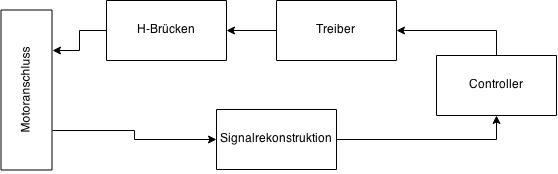
\includegraphics[width=0.8\textwidth,clip,trim=0mm 0mm 0mm 0mm]
   	{\EtPath/Bilder/Blockschaltbild_BLDC.jpg}
   	\centering
   	\caption{Blockschaltbild des BLDC-Boards}
   	\label{abb:BlockschaltbildBLDC}
\end{figure}\\
In der Abbildung \ref{abb:BlockschaltbildBLDCPhoto} ist die Realisierung der Blöcke ersichtlich. 
Dabei ist der erste Kasten der Anschluss des Motors, der zweite die H-Brücken, der dritte der 
Treiber, der vierte die Signalrekonstruktion und der fünfte Teil ist der Controller, auf dem 
die Firmware läuft.
\begin{figure}[h!]
   	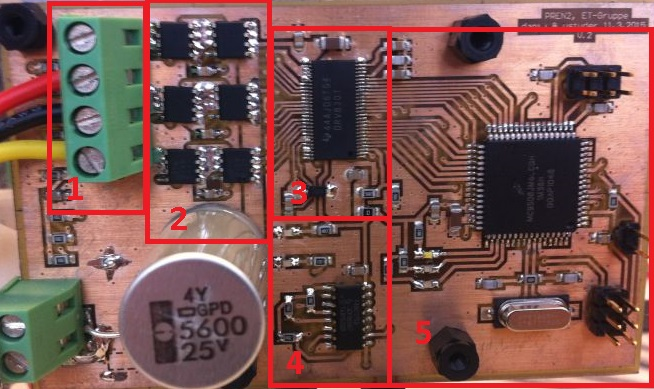
\includegraphics[width=0.8\textwidth,clip,trim=0mm 0mm 0mm 0mm]
   	{\EtPath/Bilder/BLDC-BoardBloecke.jpg}
   	\centering
   	\caption{Blockschaltbild des BLDC-Boards}
   	\label{abb:BlockschaltbildBLDCPhoto}
\end{figure}

\ifSTANDALONE
\subsection{Kommutierung}
\fi
\ifEMBED
\paragraph{Kommutierung}$~~$\vspace{2mm}\\
\fi
Der Motor wird mit drei Halbbrücken kommutiert. Für die Ansteuerung der MOSFET 
wird ein Predriver DRV8301 von Texas Instruments eingesetzt. Die Halbbrücken 
werden einzeln vom Controller geschalten. Damit nur ein 
PWM\footnote{\textbf{P}ulse \textbf{W}idth \textbf{M}odulation}-Signal erzeugt 
werden muss, werden die Ansteuerleitungen mittels Widerständen mit dem 
PWM-Signal verbunden. Werden die Ansteuerungen vom Controller nicht aktiv 
getrieben, liegt die PWM an. Die Konfiguration der Predrivers erfolgt über SPI. 

\ifSTANDALONE
\subsection{Phasendetektion}
\fi
\ifEMBED
\paragraph{Phasendetektion}$~~$\vspace{2mm}\\
\fi
Die Phasendetektion besteht aus Sternpunktnachbildung, Komparator und 
Synchronisation. Die Sternpunktnachbildung erzeugt einen virtuellen Sternpunkt 
mit Hilfe eines Widerstandsnetzwerkes und eines Tiefpassfilters. Die einzelnen 
Phasenspannungen werden mit diesem virtuellen Sternpunkt verglichen. Mit einem 
Flipflop wird das Signal mit der PWM Synchronisiert. 

\ifSTANDALONE
\subsection{Controller}
\fi
\ifEMBED
\paragraph{Controller}$~~$\vspace{2mm}\\
\fi
Als Controller kommt ein HC9S08JM60 der Firma Freescale zum Einsatz. Der Takt 
wird mittels Quarz mit 12MHz erzeugt. Um den aktuellen Betriebsszustand 
anzuzeigen, stehen drei LED zur Verfügung. 

\ifSTANDALONE
\subsection{Speisung}
\fi
\ifEMBED
\paragraph{Speisung}$~~$\vspace{2mm}\\
\fi
Die Eingangsspannung wird mittels eines optional bestückbaren Filters von 
Murata gefiltert. Der Predriver wird direkt mit dieser gefilterten Speisung 
betrieben. Mit dem im Predriver integrierten Step-Down-Converter wird eine 
Spannung von 3.3V erzeugt. Für Varianten mit hoher Betriebsspannung (>30V) 
wird der Komparator der Phasendetektion über einen diskret aufgebauten 
Spannungsregler mit einer Spannung von 30V versorgt. 

